\section{Evaluation}
\label{sec:experiments}

%Evaluate \nfactor system.

%\chuan{remember to show how many lines of code or other overhead needed for implementing NFV anew on the actor framework}

We evaluate \nfactor framework using three Dell R430 Linux servers, containing 20 logical cores, 48GB memory and 2 Intel X710 10Gb NIC. The Dell servers are connected through a 10GB switch. We use one server to run traffic generators and six virtual switches, which are capable of generating 64 byte data packets at almost 14Mpps, achieve line-rate throughput. We use the reset of the two servers to run runtimes.

To evaluate the performance of \nfactor, we implement 3 customized NF modules using the API provided by \nfactor~framework, the 3 NF modules are flow monitor, firewall and HTTP parser. The flow monitor updates an internal counter when it receives a packet. The firewall maintains several firewall rules and checks each received packet against the rule. If the packet matches the rule, a tag in the flow state is flipped and later packets are automatically dropped. The firewall also records the connection status of a flow in the flow state. For the HTTP parser, it parses the received packets for the HTTP request and responses. The requests, responses and the HTTP method are saved in the flow state. %Throughout the evaluation, we use a service chain consisting of  ``flow monitor$\rightarrow$firewall$\rightarrow$http parser'' as the service chain. We generate evaluation traffic using the BESS's FlowGen module and we directly connect the FlowGen module to the external input port of the virtual switch.

%Table goes  here to explain the functionalities of the NF modules.
The rest of the section tries to answer the following questions. \textit{First, } what is packet processing throughput of~\nfactor, does it scales well? \textit{Second,} how good is the flow migration performance of~\nfactor when compared with existing works like OpenNF? \textit{Third,} how is the performance of flow replication? \textit{Fourth,} how good is~\nfactor's dynamic scaling algorithm performs. The section concludes with the performance of the unique applications that are enabled through~\nfactor's distributed flow migration.

%how well can~\nfactor~scales, in terms of the number of runtimes running inside the system? (Sec.~\ref{sec:normal})

%what is the packet processing capacity of \nfactor~framework? (Sec. \ref{sec:ppc}) \textit{Second, } how well is \nfactor~scales, both in terms of the number of worker threads used by a runtime and the number of runtimes running inside the system? (Sec. \ref{sec:ppc}) \textit{Third, } how good is the flow migration performance of \nfactor~framework when compared with existing works like OpenNF? (Sec. \ref{sec:fmp}) \textit{Fourth, } what is the performance overhead of flow state replication and does the replication scale well? (Sec. \ref{sec:rp})

\subsection{Packet Processing Throughput}
\label{sec:ppc}

\begin{figure}[!t]
	\centering
	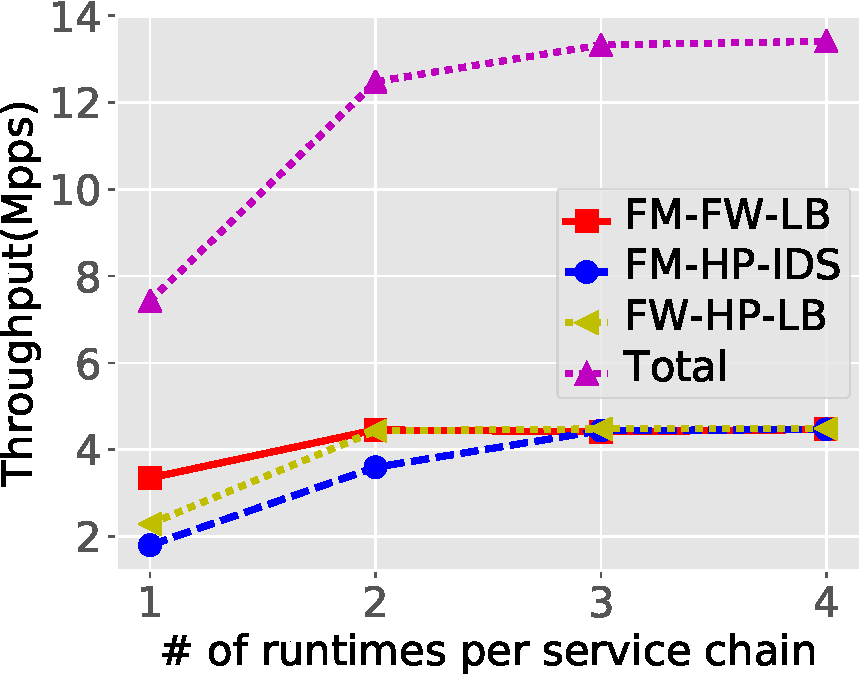
\includegraphics[width=\columnwidth]{figure/revised-throughput-test.pdf}
	\caption{The packet processing throughput using different number of runtimes. The runtimes are configured with different NFs and different service chains.
  \textbf{FM}: Flow Monitor. \textbf{HP}: HTTP Parser. \textbf{FW}: Firewall.}
\label{fig:normal-case-eval}
\end{figure}


 %\begin{figure}[!t]
%	\begin{subfigure}[t]{0.49\linewidth}
%		\centering
%		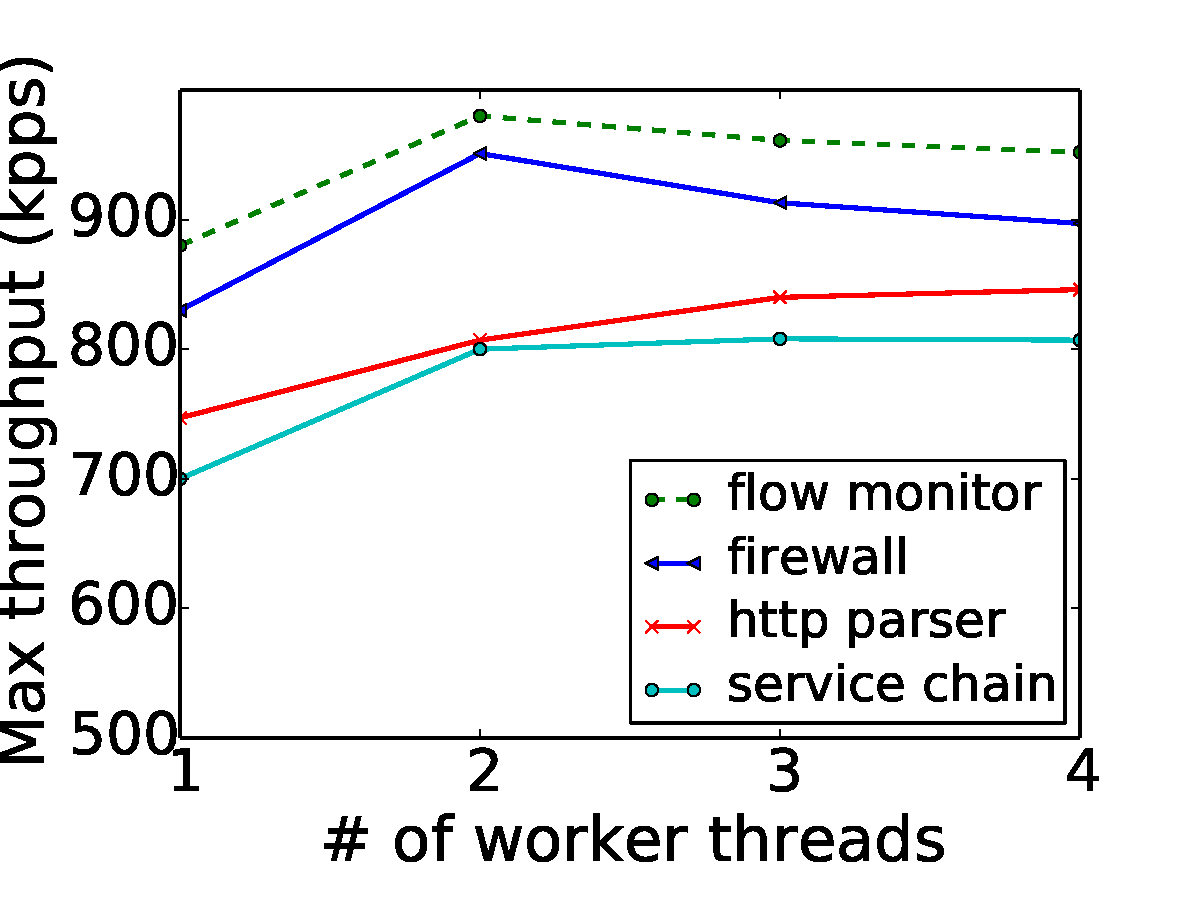
\includegraphics[width=\columnwidth]{figure/nf_throughput_evaluation.pdf}
%		\caption{Packet processing capacity of a single \nfactor~runtime system running with different number of worker threads.}\label{fig:normal-performance} \end{subfigure}\hfill
%	 \begin{subfigure}[t]{0.49\linewidth}
%		\centering
%		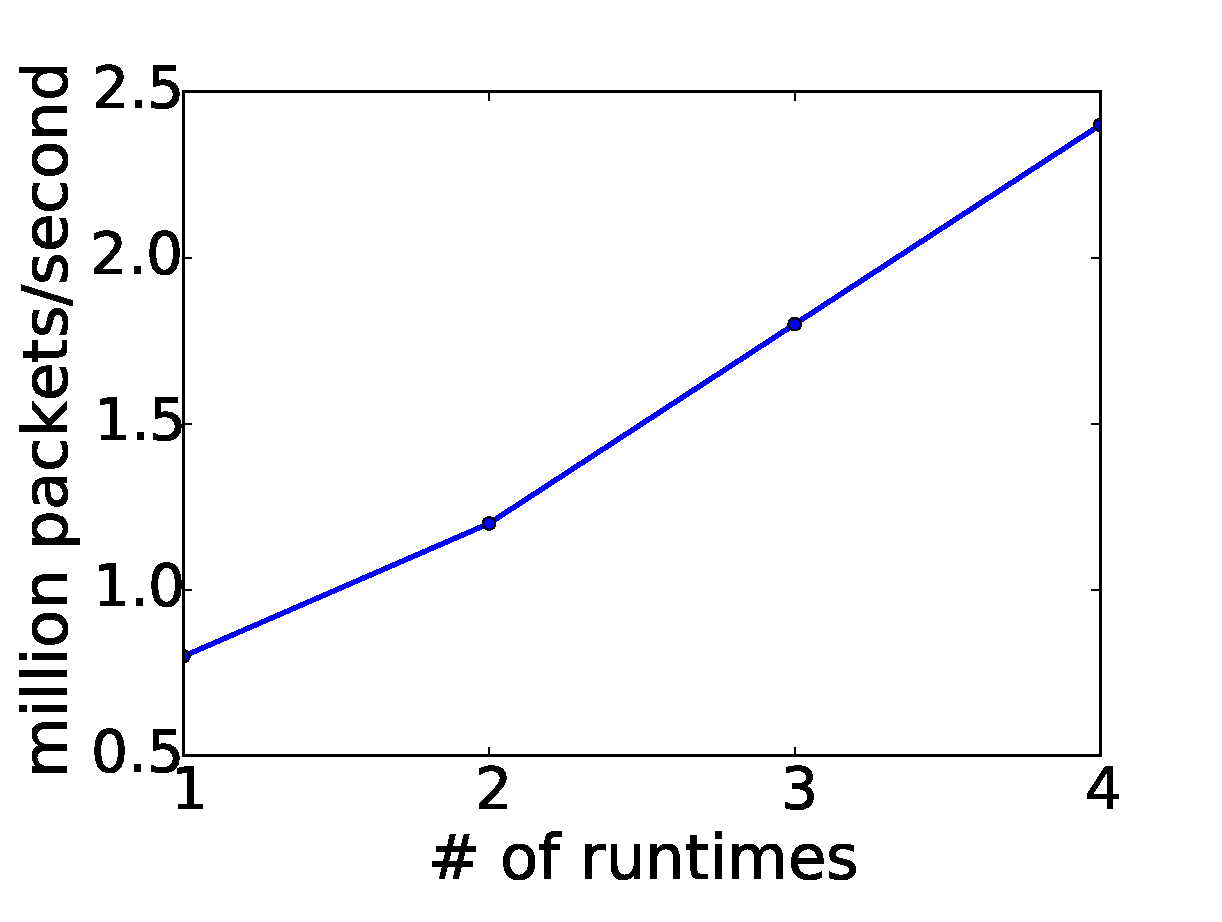
\includegraphics[width=\columnwidth]{figure/runtime_pktthroughput.pdf}
%		\caption{Aggregate packet processing capacity of several \nfactor~runtimes.}\label{fig:scalability-performance}
%	 \end{subfigure}
%\caption{The performance and scalability of \nfactor~runtime, without enabling flow migration }
%\label{fig:performance}
%\end{figure}

Figure \ref{fig:normal-case-eval} illustrates the packet processing throughput using differnt number of runtimes. The traffic generators generates flows each lasts for 10 second with a 20 pps (packet per second) flow rate. The packet size is 64 byte. We increase the number of concurrently generated flows to generate packets at around 14Mpps, reaching NIC line-rate. We set up different number of runtimes and configure runtimes with different service chains and calculate the cumulative packet rate from all the runtimes. From \ref{fig:normal-case-eval}, we can see that the runtime in~\nfactor can scale almost linearly and achieve almost line-rate processing when scaled up to 9 runtimes. Therefore,~\nfactor has good packet processing throughput and can satisfy the stringent requirement of modern NFV system.

% reach   with a uniform We can see that the packet processing throughput scales almost linearly as the number of runtime increases, until normal case performance of running \nfactor~framework. Each flow in the generated traffic has a 10 pps (packet per second) per-flow packet rate. We vary the number of concurrently generated flows to produce varying input traffics. In this evaluation, we gradually increase the input packet rate to the \nfactor~cluster and find out the maximum packet rate that the \nfactor~cluster can support without dropping packets. In figure \ref{fig:normal-performance}, the performance of different NF modules and the service chain composed of the 3 NF modules are shown. Only one \nfactor~runtime is launched in the cluster. It is configured with different number of worker threads. In figure \ref{fig:scalability-performance}, we create different number of \nfactor~runtimes and configure each runtime with 2 worker threads. Then we test the performance using the entire service chain.

%From figure \ref{fig:normal-performance}, we can learn that the packet throughput decreases when the length of the service chain is increased. Another important factor to notice is that the \nfactor~runtime does not scale linearly as  the number of worker threads increases. The primary reason is that inside a \nfactor~runtime, there is only one packet polling thread. As the number of input packets increases, the packet polling thread will eventually become the bottleneck of the system. However, \nfactor~runtime scales almost linearly as the total number of \nfactor~runtimes increases in the cluster. When the number of runtimes is increased to 4 in the system, the maximum packet throughput is increased to 2.4M pps, which confirms to the line speed requirement of NFV system.

\subsection{Flow Migration Performance}
\label{sec:fmp}

 \begin{figure}[!t]
	\begin{subfigure}[t]{0.49\linewidth}
		\centering
		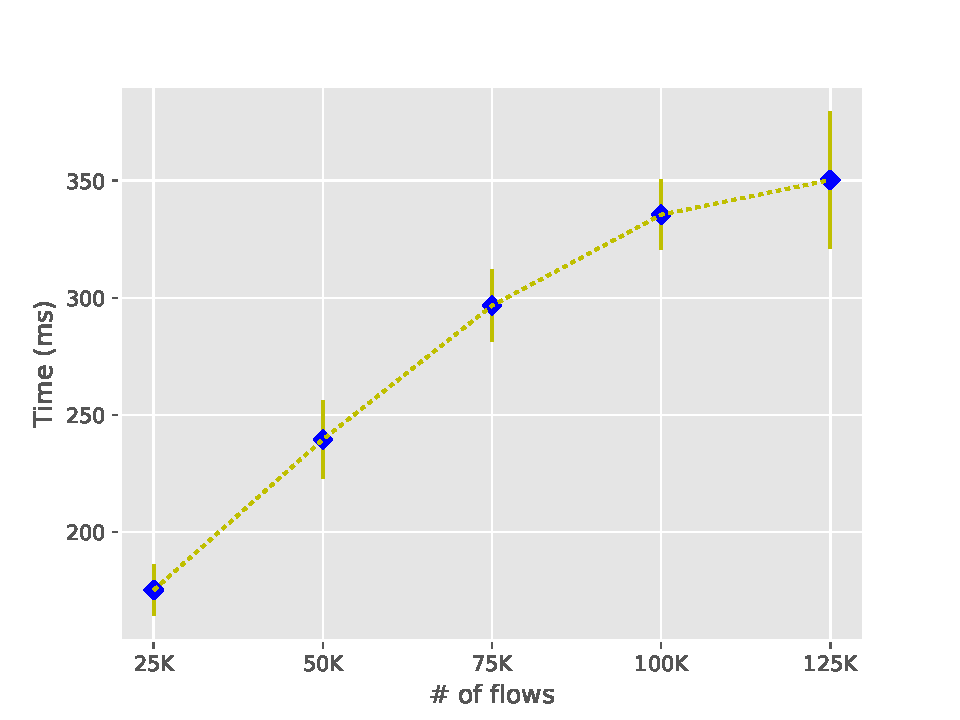
\includegraphics[width=\columnwidth]{figure/Migration.pdf}
		\caption{}\label{fig:tot-mig} \end{subfigure}\hfill
	 \begin{subfigure}[t]{0.49\linewidth}
		\centering
		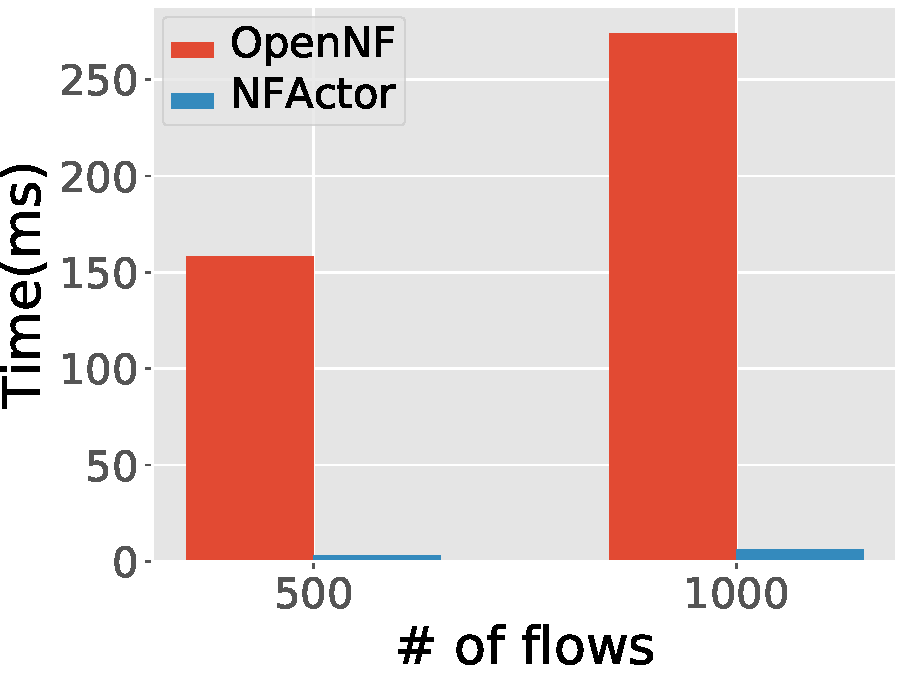
\includegraphics[width=\columnwidth]{figure/Compare.pdf}
		\caption{}\label{fig:compare-opennf}
	 \end{subfigure}
\caption{ (a) The total time to migrate different numbers of flows concurrently on three runtimes. (b) The flow migration performance of NFActor. Each flow in NFActor runtime goes through the service chain consisting of the 3 customzied NF modules. OpenNF controlls PRADS asset monitors. The flow packet rate is 20pps.}
\label{fig:mig-perf}
\end{figure}

To evaluate~\nfactor's distributed flow migration performance, we configure the three runtimes on each server. Each runtime is configured with the firewall$\rightarrow$http parser service chain. The traffic generators generate flows at 20pps and the virtual switch are only configured to generate output flow packets to runtimes on the first server, therefore each runtime on the first server processes approximately the same number of flows. After the traffic stabilizes, the coordinator concurrently initiates three migrations, asking each runtime on the first runtime to migrate all of its flows to the pair runtime on the second server.

Figure~\ref{fig:tot-mig} demonstrates average flow migration completion time calculated for all three pairs of runtimes. We can see that~\nfactor~achieves excellent flow migration performance, even when migrating more than 300000 flows, with 6Mpps processing throughput. Also, the migration are concurrently executed among three pairs of runtimes, further proving the effectiveness of \nfactor's distributed flow migration. The key reason that~\nfactor is able to achieve such a good flow migration performance is because (i) flow states are directly copied to remote actor messages without the need for serialization and deserialization and (ii) remote actor messages are directly encapsulated in L2 network packet and transmitted with high-performance packet I/O.

Finally, we compare the flow migration performance of \nfactor~against OpenNF \cite{gember2015opennf}. We generate the same number of flows to both \nfactor~runtimes and NFs controlled by OpenNF and calculate the total time to migrate these flows. The evaluation result is shown in figure \ref{fig:compare-opennf}. Under both settings, the performance of~\nfactor is much better than OpenNF. Even though this is not a fair comparison, as OpenNF uses legacy NFs while~\nfactor relies on newly implemented NFs, one can still get to know the good performance achieved by~\nfactor.

%the migration completion time of \nfactor~is more than 50\% faster than OpenNF.  This performance gain primarily comes from the simplified migration protocol design with the help of actor framework. In \nfactor, a flow migration process only involves transmitting 3 request-responses. Under light workload, the flow migration can complete within several hundreds of microseconds. Under high workload, \nfactor~runtime system controls the maximum number of concurrent migrations to control the migration workload, which may increase the migration performance as indicated in figure \ref{fig:avg-time-batch-mig}. All of these factors contribute to the improved flow migration performance of \nfactor~framework.

%three runtimes and migrate flows from one runtime on the firs

%We present the evaluation result of flow migration in this section. In order to evaluate flow migration performance, we initialize the cluster with 2 runtimes running with 2 worker threads and then generate flows to one of the runtimes. Each flow is processed by the service chain consisting of all the 3 NF modules. We generate different number of flows, each flow has the same per-flow packet rate. In order to see how the evaluation performs under different per-flow packet rate, we also tune the per-flow packet rate with 10pps, 50pps and 100pps. When all the flows arrive on the migration source runtime. The migration source runtime starts migrating all the flows to the other runtime in the cluster. We calculate the total migration time and the average per-flow migration time. In order to control the workload during the migration, the runtime only allows 1000 concurrent migrations all the time. The result of this evaluation is shown in figure \ref{fig:mig-perf}.

%We can see that as the number of migrated flows increase, the migration completion time increases almost linearly. This is because the average flow migration time remains almost a constant value and the runtime controls the maximum number of concurrent migrations. Note that when the system is not overloaded at all (100 flows), the average flow migration completion time is as small as 636us.

%When the per-flow packet rate is 100pps, the maximum number of flows that we use to evaluate the system is 6000. Continuing the evaluation with 8000 and 10000 flows just overloads the runtime as shown in figure \ref{fig:normal-performance}.

 %\begin{figure}[!t]
 %\begin{subfigure}[t]{0.49\linewidth}
%		\centering
%		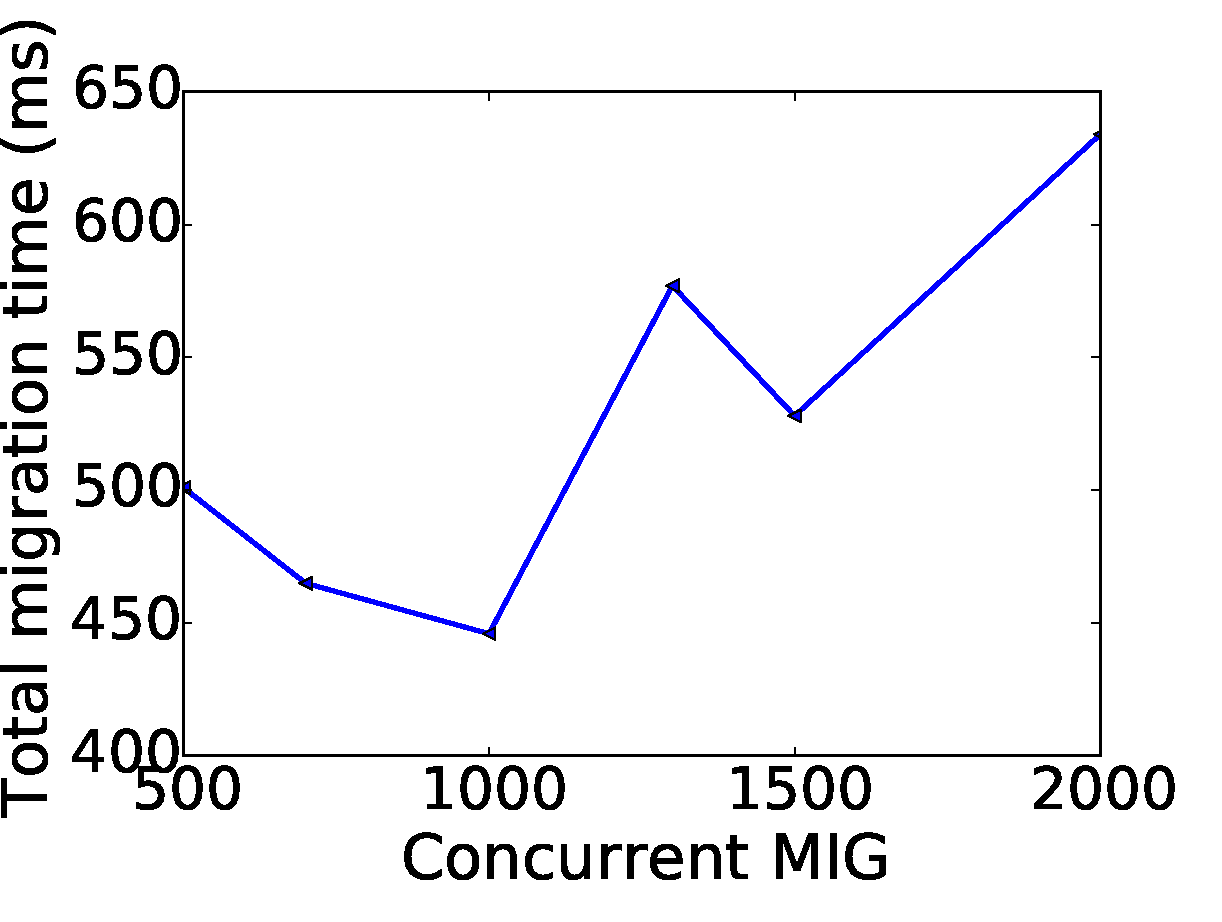
\includegraphics[width=\columnwidth]{figure/vary_batch_tot_migration_time.pdf}
%		\caption{The total time to migrate all the flows when changing the maximum concurrent migrations.}\label{fig:avg-time-batch-mig}
%	 \end{subfigure}\hfill
%	 \begin{subfigure}[t]{0.49\linewidth}
%	\centering
%		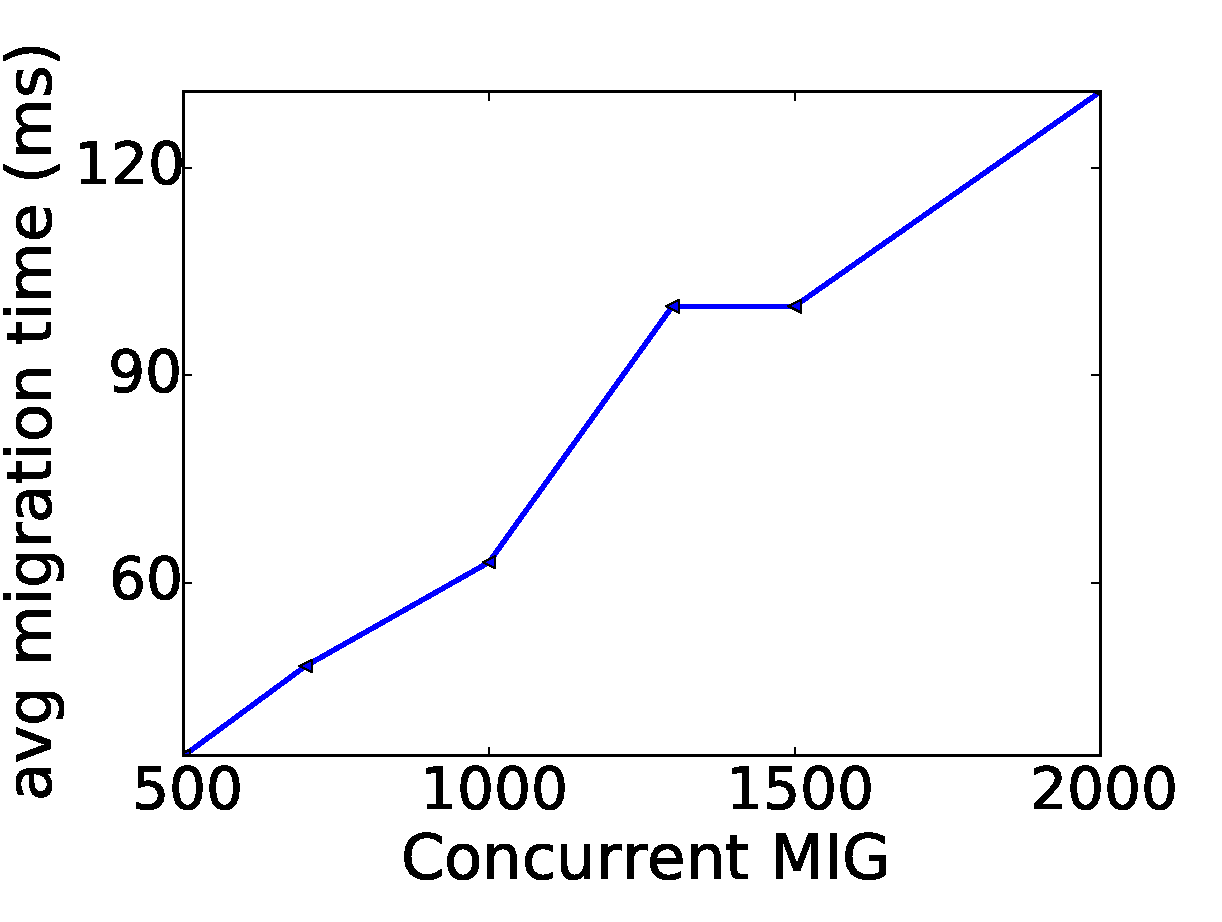
\includegraphics[width=\columnwidth]{figure/vary_batch_avg_migration_time.pdf}
%		\caption{The average flow migration time of a single flow when changing the maximum concurrent migrations.}\label{fig:avg-mig-batch} \end{subfigure}
%	\caption{The flow migration performance of \nfactor~when changing the maximum concurrent migrations.}
%\label{fig:mig-perf}
%\end{figure}

%Since we control the number of concurrent migrations, we also want to see what happens if we change the number of concurrent migrations. We generate 6000 flows, each with 50 pps per-flow packet rate, and change the the number of concurrent migrations. The result of this evaluation is shown in fig \ref{fig:mig-perf}. As we can see from fig \ref{fig:avg-mig-batch}, increasing the maximum concurrent migrations increase the average flow migration completion time. However, whether the total flow migration completion time increased depends on the total number of flows that wait to be migrated. From the result of fig \ref{fig:avg-time-mig}, the choice of 1000 concurrent migrations sits in the sweat spot and accelerates the overall migration process.

 %\begin{figure}[!t]
%		\centering
%		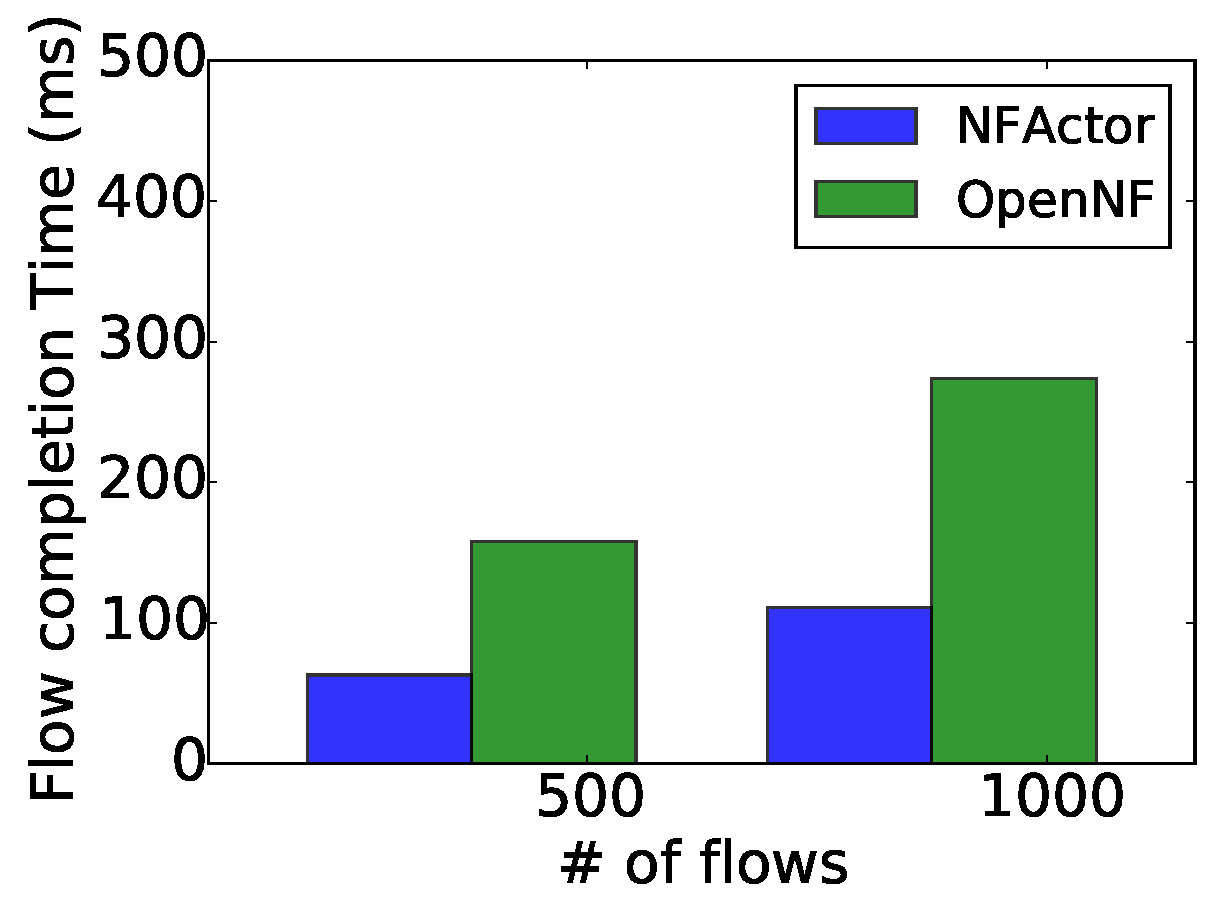
\includegraphics[width=0.6\columnwidth]{figure/opennf_nfactor_cmpFlowtime.p%df}
%		\caption{The flow migration performance of \nfactor. Each flow in \nfactor~runtime goes through the service chain consisting of the 3 customzied NF modules. OpenNF controlls PRADS asset monitors.}
%\label{fig:compare-opennf}
%\end{figure}

%Finally, we compare the flow migration performance of \nfactor~against OpenNF \cite{gember2015opennf}. We generate the same number of flows to both \nfactor~runtimes and NFs controlled by OpenNF and calculate the total time to migrate these flows. The evaluation result is shown in figure \ref{fig:compare-opennf}. Under both settings, the migration completion time of \nfactor~is more than 50\% faster than OpenNF.  This performance gain primarily comes from the simplified migration protocol design with the help of actor framework. In \nfactor, a flow migration process only involves transmitting 3 request-responses. Under light workload, the flow migration can complete within several hundreds of microseconds. Under high workload, \nfactor~runtime system controls the maximum number of concurrent migrations to control the migration workload, which may increase the migration performance as indicated in figure \ref{fig:avg-time-batch-mig}. All of these factors contribute to the improved flow migration performance of \nfactor~framework.

\subsection{Replication Performance}
\label{sec:rp}

 \begin{figure}[!t]
 \begin{subfigure}[t]{0.49\linewidth}
		\centering
		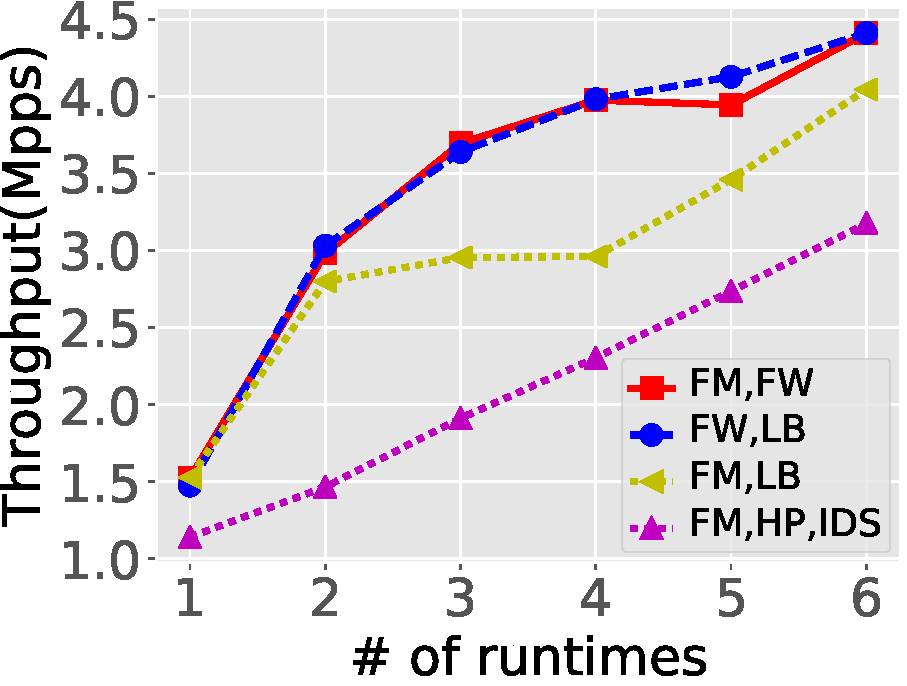
\includegraphics[width=\columnwidth]{figure/ReplicaTP.pdf}
		\caption{The packet throughput of a \nfactor~cluster when replication is enabled. }\label{fig:rep-scale}
	 \end{subfigure}\hfill
	 \begin{subfigure}[t]{0.49\linewidth}
	\centering
		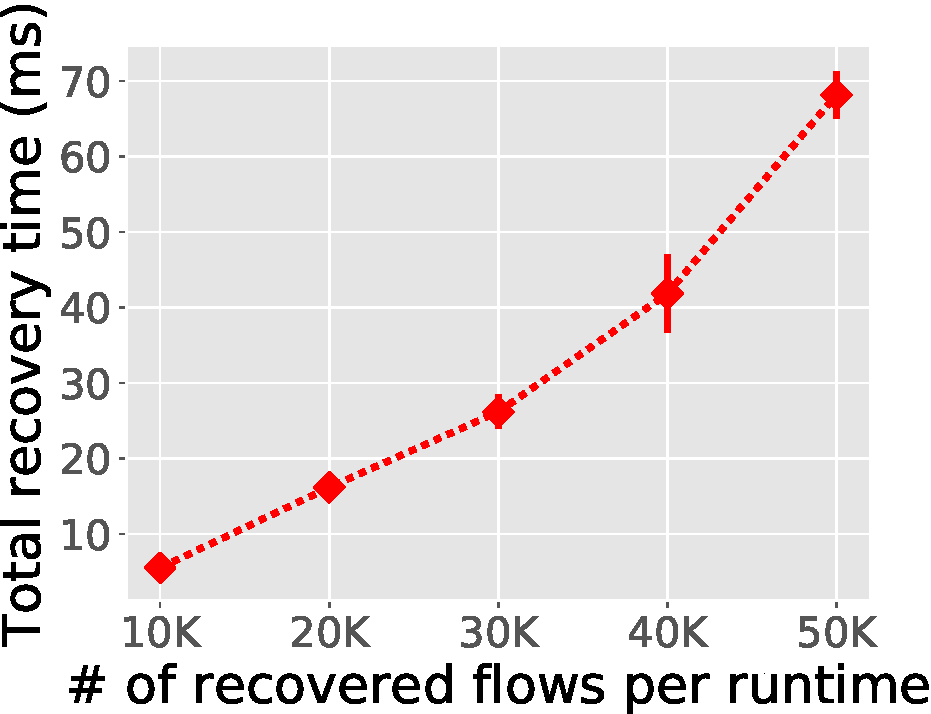
\includegraphics[width=\columnwidth]{figure/Recover.pdf}
		\caption{The recovery time of three failed runtimes under different settings. The tuple on the $x$ axis represents the number of the runtime used in the evaluation and the total input packet rate. }\label{fig:rep-recovery} \end{subfigure}
	\caption{The flow migration performance of \nfactor}
\label{fig:rep-perf}
\end{figure}

To evaluate the packet processing throughput of~\nfactor's flow replication, we configure the virtual switch to generate output packets to runtimes on the first server. For each runtime on the first server, we configure a replica runtime on the second server, and let each runtime replicate its flows to the corresponding replica runtime. We calculate the cumulative packet processing throughput during flow replication. The result is shown in Figure~\ref{fig:rep-scale}. We can see that the scalability during flow replication is not as good as the result achieved when replication is disabled. The replication throughput can achieve an almost linear scalability when there are smaller than four runtimes running in a single server, but the scalability starts to degrade when more runtimes are used. The primary reason is because the bandwidth consumption on the L2 network is way higher than normal case evaluation. To ensure output-commit property, for each input packet, the runtime generates at least two output packets, containing the flow state and the output packet processed by the flow actors.

~\nfactor replicates the flow state for each processed packet using a reliable message passing module. The number of transmitted packets by the reliable message passing module is actually two times the number of the input packets. To reliably transmit flow state and the processed packet, the runtime also needs to add a header for each remote actor message, which is 52 byte long in our implementation. All these reasons contribute to a much larger bandwidth that are actually delivered over the network, which may result in potential packet drops.

In this section, we present the flow replication evaluation result. In our evaluation, the actor creates a flow snapshot for every 10 flow packets that it has processed. Then it sends the flow state snapshot to the replica storage. In this evaluation, we first generate flows to the \nfactor~cluster to test the maximum throughput of a \nfactor~cluster when enabling replication. Then we calculate the recovery time of failed \nfactor~runtime. The recovery time is the from time that the controller detects a \nfactor~runtime failure, to the time that the recovered \nfactor~finishes replaying all of its replicas and responds to the controller to rejoin the cluster. Through out this evaluation, the runtime uses the service chain consisting of the 3 NF modules to process the flow. The result of the evaluation is shown in figure \ref{fig:rep-perf}.

In figure \ref{fig:rep-scale}, we can see that there is an obvious overhead to enable replication on \nfactor~runtimes. The overall throughput when replication is enabled drops around 60\%. This is due to the large amount of replication messages that are exchanged during the replication process. Internally, the replication messages are sent over Linux kernel networking stack, which involves data copy and context switching, thus increasing the performance overhead of using replication. However, the overall throughput when replication is enabled could scale to 850K pps when 4 runtimes are used, which is enough to use in some restricted settings.

Finally, figure \ref{fig:rep-recovery} shows the recovery time of \nfactor~runtime when replication is enabled. We found that the recovery time remains a consistent value of 3.3s, no matter how many runtimes are used or how large the input traffic is. The reason of this consistent recovery time is that the \nfactor~runtime maintains one replica on every other \nfactor~runtimes in the cluster. During recovery, several recovery threads are launched to fetch only one replica from another runtime. Then each recovery thread independently recovers actors by replaying its own replica. In this way, the recovery process is fully distributed and scales well as the number of replica increases. Note is that the average time it takes for a recovered runtime to fetch all the replicas and recover all of its actors is only 1.2s. So actually around 2.1s is spent in container creation and connection establishment.

\begin{figure}[!h]
	\centering
	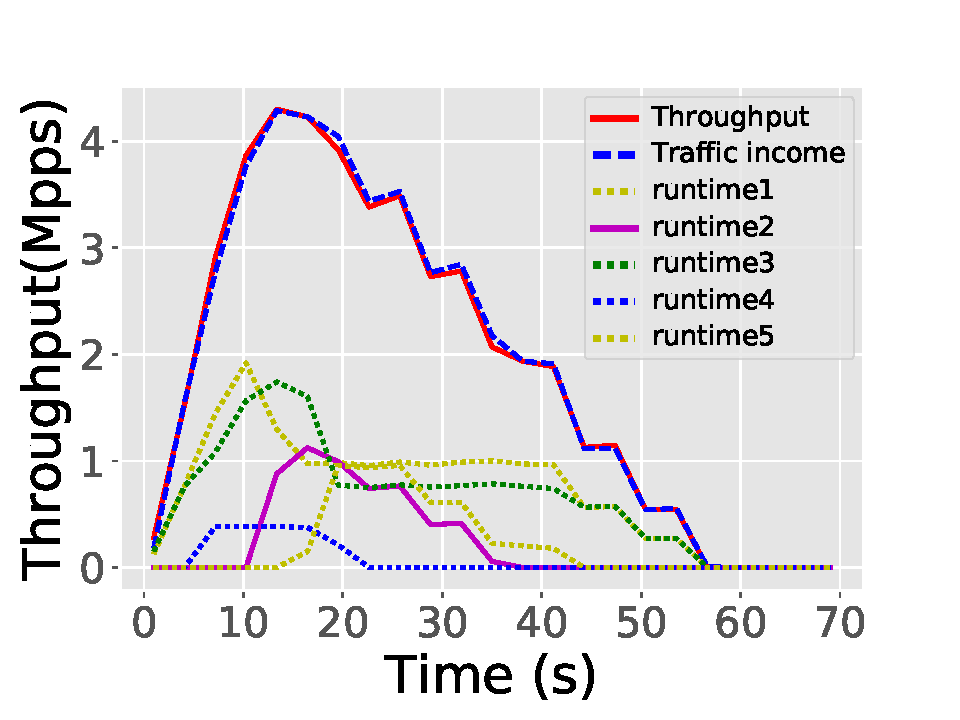
\includegraphics[width=\columnwidth]{figure/Scale.pdf}
	\caption{The packet processing throughput using different number of runtimes. The runtimes are configured with different NFs and different service chains.
  \textbf{FM}: Flow Monitor. \textbf{HP}: HTTP Parser. \textbf{FW}: Firewall.}
\label{fig:normal-case-eval}
\end{figure}

\begin{figure*}[!ht]
\begin{subfigure}[t]{0.33\linewidth}
   \centering
   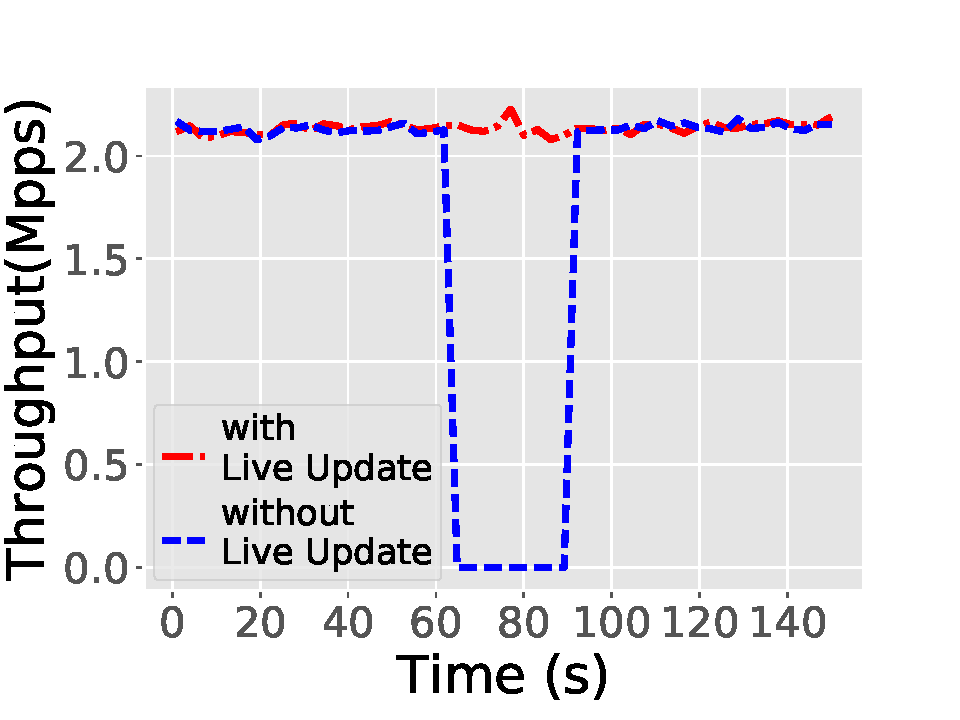
\includegraphics[width=\columnwidth]{figure/Dynamic.pdf}
   \caption{The packet throughput of a \nfactor~cluster when replication is enabled. }\label{fig:rep-scale}
  \end{subfigure}\hfill
  \begin{subfigure}[t]{0.33\linewidth}
 \centering
   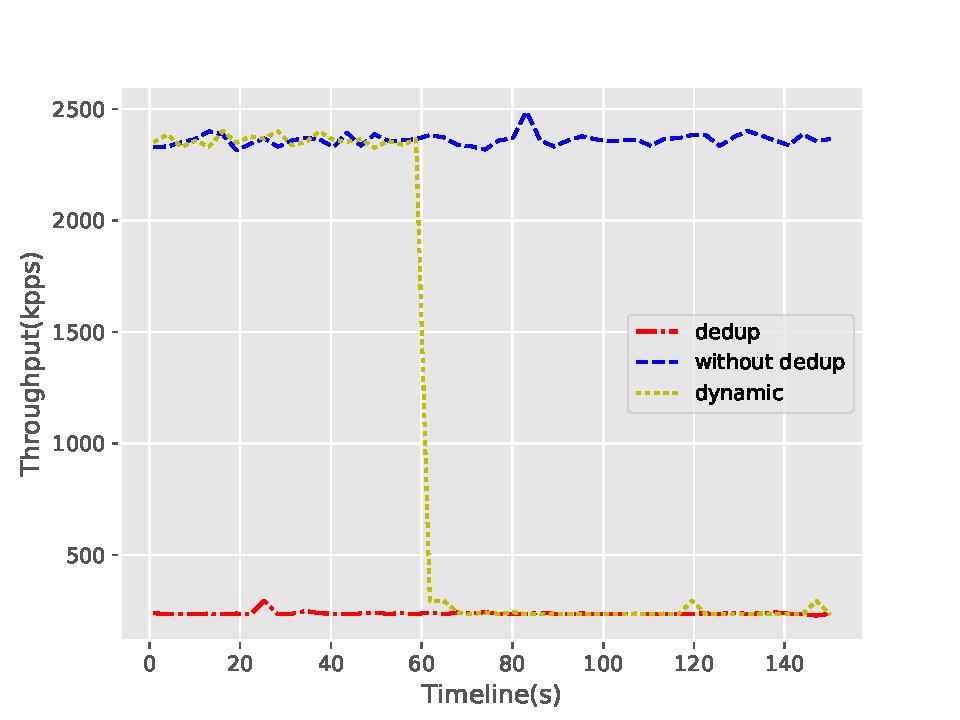
\includegraphics[width=\columnwidth]{figure/Dedup.pdf}
   \caption{The recovery time of three failed runtimes under different settings. The tuple on the $x$ axis represents the number of the runtime used in the evaluation and the total input packet rate. }\label{fig:rep-recovery} \end{subfigure}\hfill
   \begin{subfigure}[t]{0.33\linewidth}
  \centering
    \includegraphics[width=\columnwidth]{figure/MPTCP.pdf}
    \caption{The recovery time of three failed runtimes under different settings. The tuple on the $x$ axis represents the number of the runtime used in the evaluation and the total input packet rate. }\label{fig:rep-recovery} \end{subfigure}
 \caption{The flow migration performance of \nfactor}
\label{fig:rep-perf}
\end{figure*}
